%%%%%%%%%%%%%%%%%%%%%%%%%%%%%%%%%%%%%%%%%%%%%%%%%%%%%%%%%%%%%%%%%
% Contents: The first start chapter
%%%%%%%%%%%%%%%%%%%%%%%%%%%%%%%%%%%%%%%%%%%%%%%%%%%%%%%%%%%%%%%%%

\chapter{Erster Start von Grisbi\label{start}}


\section{Assistent Basiskonfiguration\label{start-first}}

Nach der Installation von Grisbi wird Ihnen die Software beim ersten Start mit drei aufeinanderfolgenden Assistenten helfen:

\begin{enumerate}
	\item Der erste Assistent \dequote{Willkommen zu Grisbi}, der nur einmal, beim ersten Start, erscheint, hilft Ihnen bei der Konfiguration der Anwendung. Sie umfasst zwei Schritte, von denen der zweite die Verwaltung der \indexword{Kontodatei}\index{Kontodatei} betrifft (automatisches Laden und Speichern, Verschlüsselung und Sicherungskopien).%The first wizard \enquote{Welcome to Grisbi!}, which will only appear once, on first launch, helps you configure the application. It comprises two steps, the second of which concerns management of the \indexword{account file}\index{account file} (automatic loading and saving, encryption and backup copies).	
	
\begin{figure}[htbp]
	\begin{center}
		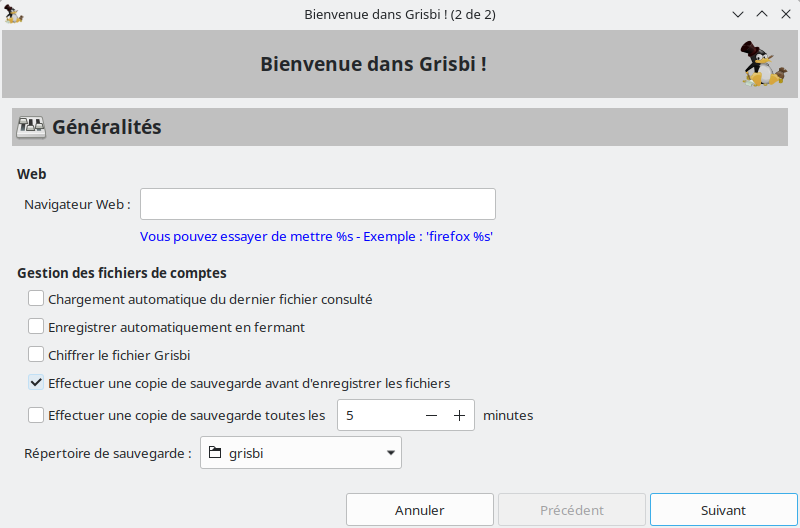
\includegraphics[width=.98\textwidth]{image/screenshot/start_first_launch}
	\end{center}
	\caption{Erstkonfiguration der Kontendatei.}
	\label{start_first_launch}
\end{figure}	
	
Es ist ratsam, die Optionen zu prüfen:%It is advisable to check the options:
	\begin{itemize}
		\item Die letzte Dateï automatisch öffnen;% Automatically load last file on startup%chargement automatique du dernier fichier consulté;
		\item Automatisch speichern;%Automatically save on exit;%enregistrer automatiquement en fermant;
		\item Vor dem Speichern eine Sicherung erstellen (standardmäßig aktiviert).%Make a backup copy before saving files (checked by default).%effectuer une copie de sauvegarde avant d'enregistrer les fichiers (coché par défaut).
	\end{itemize}
\end{enumerate}

\minisec{\textcolor{red}{\strong{Achtung:}}}
Die Grisbi-Entwickler empfehlen, die Option \menu{Datei verschlüsseln} aus den folgenden Gründen nicht zu verwenden:%The Grisbi developers recommend that you do not use the \menu{Encrypt Grisbi file} option for the following reasons:
\begin{itemize}
	\item Es gibt keine Methode zur Wiederherstellung einer verschlüsselten Datei, deren Passwort verloren gegangen ist;%there is no method for recovering an encrypted file whose password has been lost;
	\item Aus einem unbekannten Grund kann die Verwendung dieser Option unter Windows dazu führen, dass die Kontendatei völlig unbrauchbar wird.%For some unknown reason, using this option on Windows can render the accounts file completely unusable.
\end{itemize}  
Es ist jedoch ratsam, regelmäßig Sicherungskopien der unverschlüsselten Datei anzufertigen, wenn Sie sie verwenden.%However, if you use it, it is advisable to make regular back-ups of the unencrypted file.

\begin{enumerate}[resume]
	\item Der zweite Assistent, \dequote{Willkommen zu Grisbi} (oder später \dequote{Assistent für eine neue Datei}), der automatisch auf den ersten folgt, umfasst sechs Schritte, die Ihnen bei der Erstellung der \indexword{Kontodatei}\index{Kontodatei} helfen.%The second wizard, \dequote{Willkommen zu Grisbi} (or later \dequote{New file Assistant}), which automatically follows the first, includes six steps to help you create the \indexword{account file}\index{account file}.%Le deuxième assistant \frquote{Bienvenue dans Grisbi !} (ou plus tard \frquote{Aide à la création d'un nouveau fichier de comptes}), qui suit automatiquement le premier, comprend six étapes qui vous aiderons à la création du \indexword{fichier de comptes}\index{fichier de comptes}.
	\item Darauf folgt automatisch der dritte Assistent, \dequote{Ein neues Konto erstellen}, der zum Erstellen des ersten Kontos verwendet wird und im Abschnitt \ref{start-newfile} unten ausführlich beschrieben wird.%This is followed automatically by the third wizard, \dequote{Create a new account}, which is used to create the first account and is described in detail in section \ref{start-newfile} below.%Puis vient automatiquement le troisième assistant \frquote{Créer un nouveau compte} qui permet de créer le premier compte et qui est décrit en détail dans la section \ref{start-newfile} ci-dessous.
\end{enumerate}

Sie können jeden Assistenten jederzeit mit der Schaltfläche \menu{Abbrechen} verlassen.

Wenn Sie den Erststart-Assistenten nicht verwenden möchten, können Sie stattdessen eine Beispieldatei verwenden (siehe Abschnitt \ref{start-example} unten).

\section{Beispieldatei\label{start-example}}

Wenn Sie Grisbi sofort benutzen wollen, ohne die komplette Einrichtung durchlaufen zu müssen, zum Beispiel um eine Vorstellung von den Möglichkeiten dieses Programms zu bekommen, können Sie die Datei \file{Example\_3.0-de.gsb} von der \lang{Sourceforge.net}\footnote{\urlSourceForgeDocumentation{}} Website im Ordner \dequote{textsf{examples}} herunterladen.

\vspacepdf{5mm}
\textbf{Notiz}: In dieser Beispieldatei sind die Namen der Zahlungsempfänger usw. reine Erfindung; jede Ähnlichkeit mit einer realen Person oder einem realen Unternehmen ist rein zufällig.%{Note}: in this example file, the names of the payees etc are pure invention; any similarity with a real person or business is entirely accidental.

\section{Erstellen einer neuen Kontodatei\label{start-newfile}}

